\documentclass[a4paper,12pt]{article}
\usepackage[utf8]{inputenc}
\usepackage[T1]{fontenc}
\usepackage[french]{babel}
\usepackage{graphicx}
\usepackage{alltt}
\usepackage{listings}
\usepackage{moreverb}
\usepackage[colorlinks=true,linkcolor=black,urlcolor=blue]{hyperref}
\usepackage{tikz}

\usetikzlibrary{mindmap,trees}
\addtolength{\hoffset}{-1cm}
\addtolength{\textwidth}{2cm}

\definecolor{rouge}{HTML}{993333} 

\title{
	\normalsize{ENSEIRB-MATMECA \\ 
	2012 - 2013 \\
	2ème année informatique} \\
	\vspace{15mm}
	\Huge{\textcolor{blue}{Projet de Système d'Exploitation }}
} 
\author{ BENOIT Amélie \\ BRISSET Clément \\ LANDEIRO DOS REIS Virgile \\ RABENJAMINA Samantha \\ RUELLE Benoît}

\date{
	\normalsize{Enseignant encadrant : François TESSIER}
}

\begin{document}

\maketitle
\clearpage
\tableofcontents
\clearpage

\section{Introduction et mise en route}
Ce projet s'inscrit dans la continuité du cours et des TDs du module de Systèmes d'exploitation. Le but de ce projet et de mettre en place une bibliothèque de gestion des threads en espace utilisateur. Celle-ci reprend le comportement de la bibliothèque existante $pthread$. 

Dans un premier temps, nous avons défini une structure représentant un thread. Nous avons ensuite implémenté les fonctions définies dans le fichier $thread.h$ donné dans l'énoncé. Dans un deuxième temps, nous avons testé cette bibliothèque sur les exemples fournis et sur d'autres, que nous avons implémentés (tris de tableaux, calcul de la somme d'un tableau). Enfin, nous avons commencé à réaliser des fonctions avancées telles que la préemption, les threads noyaux et la fonction cancel. 



\section{Développement de la bibliothèque}
<<<<<<< HEAD
La première étape a été de récupérer le squelette du code de la bibliothèque de
thread et de coder les fonctions nécessaires à son fonctionnement. Cette partie
explique les choix qui ont été faits, ainsi que les problèmes rencontrés et la
façon dont nous les avons résolus.
=======
La première étape a été de récupérer le squelette du code de la bibliothèque de thread et de coder les fonctions nécessaires à son fonctionnement. Cette partie explique les choix qui ont été faits, ainsi que les problèmes rencontrés et la façon dont nous les avons résolus.
>>>>>>> b8f2cb4a0a18f30b59a4153afd67045492348297

\subsection{Choix de programmations}

L'initialisation de la bibliothèque est implicite et ne nécessite pas d'être
faite manuellement par le code client. En effet, des fonctions \verb!__init()!
(resp. \verb!__destroy()!) avec l'attribut \verb!__attribute__((constructor))!
(resp. \verb!__attribute__((destructor))!) fourni par gcc permettent de
réaliser les initialisations (resp. le nettoyage) nécessaires au bon
fonctionnement.

Les listes de \verb!sys/queue.h! empruntées à BSD ont été retenues pour leur
simplicité d'utilisation et leur "légèreté". Les files et listes doublement
chaînées permettent des ajouts et suppressions en temps constant et ces
oppérations peuvent être réalisées pendant leur parcours
(\verb!*_FOREACH_SAFE!).


\subsection{Le cas du thread principal}

<<<<<<< HEAD
La gestion du thread principal nécessite des opérations différentes des autres
threads notamment lors de la libération de ressource ou de l'ordonnancement. En
effet, les tests qui nous sont fournis demandent à ce que le thread principal
fasse des \verb!yield! vers des fils et un fils doit faire des \verb!yield!
vers le thread principal (cf. \verb!02-switch.c!). De plus, le thread principal
doit pouvoir être utilisé dans la fonction \verb!thread_join()! tout en
permettant aux autres threads de continuer à utiliser \verb!yield!.
=======
La gestion du thread principal nécessite des opérations différentes des autres threads notamment lors de la libération de ressources ou de l'ordonnancement. En effet, les tests qui nous sont fournis demandent à ce que le thread principal fasse des \verb!yield! vers des fils et un fils doit faire des \verb!yield! vers le thread principal (cf. \verb!02-switch.c!). De plus, le thread principal doit pouvoir être utilisé dans la fonction \verb!thread_join()! tout en permettant aux autres threads de continuer à utiliser \verb!yield!.
>>>>>>> b8f2cb4a0a18f30b59a4153afd67045492348297


\section{Objectifs avancés}
\subsection{Les threads noyaux}
Dans cette partie, afin d'alléger les phrases, une tâche est synonyme de thread utilisateur (que l'on doit distinguer des threads noyaux).

\subsubsection{Aperçu du fonctionnement}

Afin d'utiliser tous les processeurs disponibles, un certain nombre (fixé à la compilation) de threads noyaux sont créés lors de l'initialisation de la bibliothèque. Ce nombre inclut le thread principal qui n'est pas distinguable des threads créés du point de vue de l'utilisateur. Les threads alors créés entrent dans une boucle infinie dans laquelle ils vont consommer des tâches à réaliser placés dans une file.

Ces tâches sont celles créées par l'utilisateur via la fonction \verb!thread_create()! de la bibliothèque. Elles sont définies par un contexte et quelques attributs sur leur état.


\subsubsection{Creation de threads noyaux}

\paragraph{Avec clone()}
Nous avons tout d'abord utilisé l'appel système \verb!clone()! avec notamment les flags \verb!CLONE_VM! (partage de la mémoire), \verb!CLONE_THREADS! (processus créés dans un même groupe de threads), etc. Cette solution a bien abouti mais nous a permis de nous rendre compte de plusieurs problèmes.

Le premier est le stockage de données propres au thread qui sont utiles pour les distinguer et rendre l'appel à \verb!thread_self()! efficace. L'idée était alors de conserver un pointeur global vers le thread utilisateur courant qui lui permettrait, lorsqu'il est exécuté sur un thread noyau, d'avoir un accès immédiat vers la structure qui le représente. Une solution (non portable) proposée par gcc est de déclarer des variables avec l'attribut \verb!__thread! mais nous ne sommes pas parvenu à obtenir le comportement souhaité car la valeur du pointeur semblait partagée entre tous les processus malgré tout. Nous avons donc changé d'approche et avons résolu notre problème en créant un tableau associant un l'identifiant d'un thread noyau (obtenu via \verb!gettid()!) à un thread utilisateur. Cette solution nécessite donc le parcours d'un tableau de taille égale au nombre de threads noyaux à chaque fois que l'on souhaite identifier quel thread utilisateur est exécuté.

Le second problème provient de glibc. En effet, lorsque l'on dit que glibc est
'thread-safe', il faut en fait comprendre 'pthread-safe'
\footnote{\url{http://sourceware.org/ml/libc-alpha/2006-01/msg00086.html}}
\footnote{\url{http://osdir.com/ml/lib.glibc.bugs/2003-01/msg00012.html}}.
Nous nous en sommes rendu compte lors d'appels intensifs vers \verb!malloc!
pour la création de threads utilisateur dans les tests comme fibonacci : nous
obtenions des corruptions du tas laissant penser que malloc n'était pas
thread-safe!  L'explication est simple : l'ensemble de glibc dépend énormément
du fonctionnement de pthread pour les applications multi-threadées et fait des
ajustements pour avoir un comportement correct dans ce type de programme. En
voulant se passer de pthread au profit d'une implémentation plus bas niveau
grâce à \verb!clone()! avec \verb!CLONE_VM!, nous contournons ces ajustements
et l'utilisation de la bibliothèque standard n'est alors plus sûre. La
corruption du tas fût corrigée avec un simple mutex placé avant chaque
\verb!malloc()! ou \verb!free()!, confirmant notre observation. Ceci est lourd
de conséquence car la même précaution doit alors être prise par l'utilisateur
et cela pour toutes les fonctions de la bibliothèque standard pouvant souffrir
d'appels concurrents!


\paragraph{Avec pthread\_create()}
Afin de supprimer la limitation précédente, nous avons remplacé l'appel à \verb!clone()! par un appel à \verb!pthread_create()!. Les mutex avant l'allocation et la libération de mémoire ont alors pu être supprimées sans faire réaparaitre de corruption et nous avons pu utiliser des \verb!pthread_key! pour stocker un pointeur vers la tâche courante et s'affranchir du parcours de tableau précédent.


\subsubsection{Ordonnancement des tâches}

L'ordonnancement de plusieurs tâches sur l'ensemble des threads noyaux est réalisé grâce aux techniques suivantes :

\paragraph{File de tâches} Les threads utilisateur sont stockés dans une file. Un mutex et un sémaphore y sont associés pour la concurrence et le signalement de nouvelles tâches enfilées respectivement.

\paragraph{Contexte d'un thread noyau} À l'initialisation, on distingue deux cas pour les threads noyaux. Le thread principal (qui est exécuté depuis le début du programme) n'est pas altéré: il continue l'exécution normale du programme dans un premier temps tandis que les threads créés attendent les premières tâches à exécuter dans une boucle infinie qui va consommer des tâches placées dans la file (fonction \verb!_clone_func()!).

\paragraph{Exécution des threads utilisateur} Pour chaque thread noyau, le thread utilisateur exécuté est responsable de l'exécution du thread utilisateur suivant. 

En fonction de la quantité de threads noyaux et de tâches, trois cas peuvent se présenter :
\begin{itemize}
	\item Si la file de tâches est vide et que le thread utilisateur courant est terminé, alors on repasse dans le contexte thread noyau pour attendre de nouvelles tâches sauf s'il l'on détecte que nous sommes le tout dernier thread exécuté auquel cas le programme termine. Dans le cas où ce thread noyau est le thread principal, on lance la fonction d'attente sur la file \verb!_clone_func()!.
	\item Sinon si la file est vide mais que le thread courant n'est pas fini, alors ne rien faire et continuer l'exécution.
	\item Sinon, la file n'est pas vide donc appeler une fonction de changement de contexte \verb!_magicswap()! détaillée plus loin.
\end{itemize}

<<<<<<< HEAD
\paragraph{Changements de contextes avec \_magicswap} Afin d'éviter qu'une même tâche soit manipulée par plusieurs threads noyaux à la fois, on associe à chacune d'elles un mutex qui doit être pris par le thread noyau avant toute opération. Un thread noyau souhaitant exécuter une tâche doit avoir pris le verrou et le conserver pendant toute l'exécution, y compris avant et après le \verb!swapcontext!.
=======
\paragraph{Changements de contextes avec \_magicswap()} Afin d'éviter qu'une même tâche soit manipulée par plusieurs threads noyaux à la fois, on associe à chacune d'elles un mutex qui doit être pris par le un thread noyau avant toute opération. Un thread noyau souhaitant exécuter une tâche doit avoir pris le verrou et le conserver pendant toute l'exécution, y compris avant et après le \verb!swapcontext!.
>>>>>>> 44202ee307b1f39e766600b4248cd1ba085d652d

Avec ce schéma et s'il l'on souhaite ne pas repasser au contexte du thread noyau pour réaliser la libération de l'ancienne tâche et le verrouillage d'une nouvelle, il faut pouvoir indiquer à une tâche sa tâche appelante afin de réaliser la libération.

Une tâche en appelant une autre doit donc préparer la tâche suivante en vérouillant son mutex, en lui indiquant qui l'a appelé, en changeant le pointeur de tâche courante du thread noyau et enfin en réalisant le changement de contexte. Une tâche venant d'être exécutée doit quant à elle récupérer son identité grâce au pointeur de tâche courante du thread noyau, libérer la tâche appelante ainsi que la replacer dans la file si elle n'est pas terminée et enfin continuer son exécution normale.


\subsection{Système de préemption}
Nous avons utilisé la fonction $ualarm$ pour envoyer un signal d'alarme $SIGALRM$ à intervalles réguliers. Ce signal est bloqué par un gestionnaire de signaux initialisé en même temps que la bibliothèque $thread.h$. Le handler correspondant à ce gestionnaire est donc appelé. 

Dans un premier temps, il passait la main du contexte courant à un contexte spécialement dédié à l'ordonnancement. Ce contexte ordonnanceur passait la main au contexte suivant de la liste $ready$.  Nous avons cependant rencontré des difficultés à implémenter la préemption de cette manière (incohérences lors des changements de contexte). De plus, cette solution ne semblait pas optimale, en raison d'un nombre élevé de changements de contextes, à la fois coûteux et peu utiles.

Par conséquent, nous avons appelé directement la fonction $thread\_yield$ dans le handler. Cette fonction prenait en compte le cas particulier du thread main. Lorsque l'on se trouvait dans le main, on passait la main au thread suivant dans la liste $ready$. Ceci causait le même problème qu'avec le contexte dédié, car à chaque fois que l'on voulait passer la main au thread suivan dans $ready$, on repassait d'abord par le main. Nous avons donc implémenté une fonction similaire à $thread\_yield$, qui évite ce problème en ne repassant plus la main au main. 

Dans le cas particulier où la liste $ready$ est vide ou ne comprend qu'un seul
thread, il n'est pas nécessaire d'avoir recours à la préemption. Il faut donc
désactiver le gestionnaire correspondant à $SIGALRM$ jusqu'à ce qu'un nouveau
thread soit inséré dans la liste.


\subsection{Définition des priorités}
Après l'implémention de la préemption, nous avons pu développer une gestion de la priorité. Deux possibilités s'offraient à nous : Round-robin et l'utilisation de plusieurs listes de priorités.

Round-robin consiste à voir la liste de thread $ready$ comme une liste circulaire. Tout nouveau processus est placé à la fin de la liste. Le processus courant est préempté après un temps d'exécution fonction de sa priorité, et passe la main au processus suivant.

L'autre algorithme consiste à créer une liste $ready$ pour chaque valeur de priorité. Les processus sont ajoutés à la liste correspondant à leur priorité lors de leur création. Les processus de priorités élevées sont exécutés plus souvent et plus longtemps que les autres. Pour cela, on exécute successivement un nombre défini de processus d'une liste $ready$, puis d'une autre.

\begin{figure}[!h]
\centering
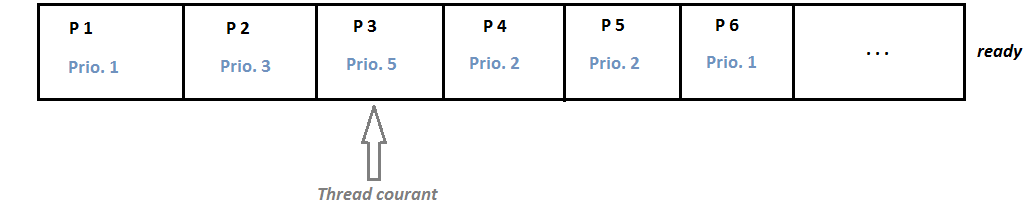
\includegraphics[width=0.9\textwidth]{round_robin.png}
\caption{Système de priorité basé sur Round-Robin}  
\label{sequence} 
\end{figure} 

\begin{figure}[!h]
\centering
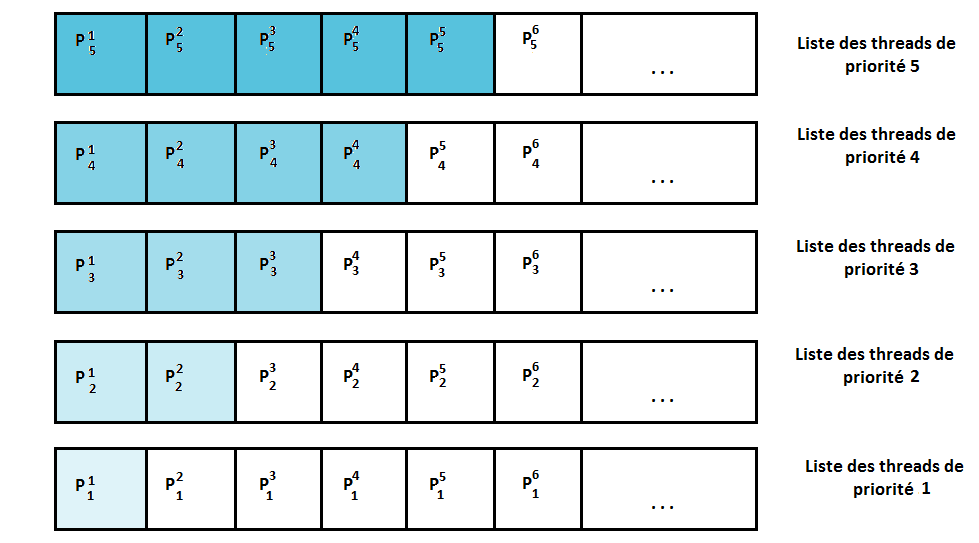
\includegraphics[width=0.9\textwidth]{queus_multi.png}
\caption{Système de priorité basé sur plusieurs listes}  
\label{sequence} 
\end{figure} 


Les deux solutions nous semblaient également efficaces (pas de famines). Nous avons cependant choisi d'implémenter Round-robin pour sa simplicité. Nous avons ajouté un champ entier $priority$ dans la structure $thread$. Plus cette priorité est élévée, plus le thread est prioritaire. Ainsi, lorsqu'un thread de $ready$ est exécuté, son temps d'exécution est proportionnel à sa priorité. Les processus de priorité s'exécutent donc plus longtemps, assurant une gestion des priorités efficace.

\subsection{Annulation de threads}
Pour l'annulation, une première implémentation à été réalisée avant la mise en oeuvre des threads noyaux. Celle-ci était alors relativement simple, 2 variables on étés rajoutés dans la structure \verb!thread! (\verb!state! et \verb!canceled!) spécifiant si l'annulation pour le thread en question est autorisée ou non, et si elle ne l'est pas, si une annulation à été demandé, car celle-ci sera effectuée lorsque le thread repassera dans l'état où une annulation est autorisé.\\

Pour celà, 2 fonctions on été implémentées :
\begin{itemize}
\item \verb!thread_cancel()! : Chargée d'annuler le thread si le thread est dans l'état\\ \verb!THREAD_CANCEL_ENABLE! ou alors de placer \verb!canceled! à 1 si il est dans l'état \verb!THREAD_CANCEL_DISABLE!. Son implémentation est voisine de celle de la fonction \verb!thread_exit()!.\\
\item \verb!thread_setcancelstate()! : Chargée de changer l'état du thread, ainsi que de l'appel de \verb!thread_cancel()! dans le cas où \verb!canceled! vaut 1 et le nouvel état est \verb! THREAD_CANCEL_ENABLE!.
\end{itemize}

Une fois les threads noyaux implémentés, le code à due être adapté, car plus rien ne garantissait la présence du thread dans la file \verb!ready! au moment de l'appel de \verb!thread_cancel()!. Celui ci peut très bien se trouver en cours d'éxécution par un thread noyaux différent. Pour éviter les problème de concurrence, il est alors apparut judicieux d'effectuer l'annulation au moment du désordonnancement: avant de replacer la tâche dans la file, on vérifie qu'elle n'a pas été annulée sinon ses ressources sont libérées.




\section{Tests de robustesse et de performance}
\subsection{Les tests de base}
\subsection{Tests implémentés}
\subsubsection{Somme des éléments d'un tableau}
\subsubsection{Les tris de tableaux}
Les algorithmes de tri de tableaux $tri rapide$ et $tri fusion$ ont été implémentées. Dans le cas du $tri rapide$, un thread est créé traîter chaque partie du tableau de part et d'autre du pivot. Pour le $tri fusion$, chaque fois qu'un tableau est divisé en deux, chaque partie est traitée par un nouveau thread.\\

%%%% resultats tests + include graphics %%%%
%\begin{figure}[H]
%\includegraphics[scale=0.4]{pouetpouet.png}
%\caption{Temps d'exécution des tests d'un tri rapide}
%\end{figure} 


\section{Conclusion}
conclu

\end{document}
